\begin{figure}[H]
\centering
\shorthandoff{<>}
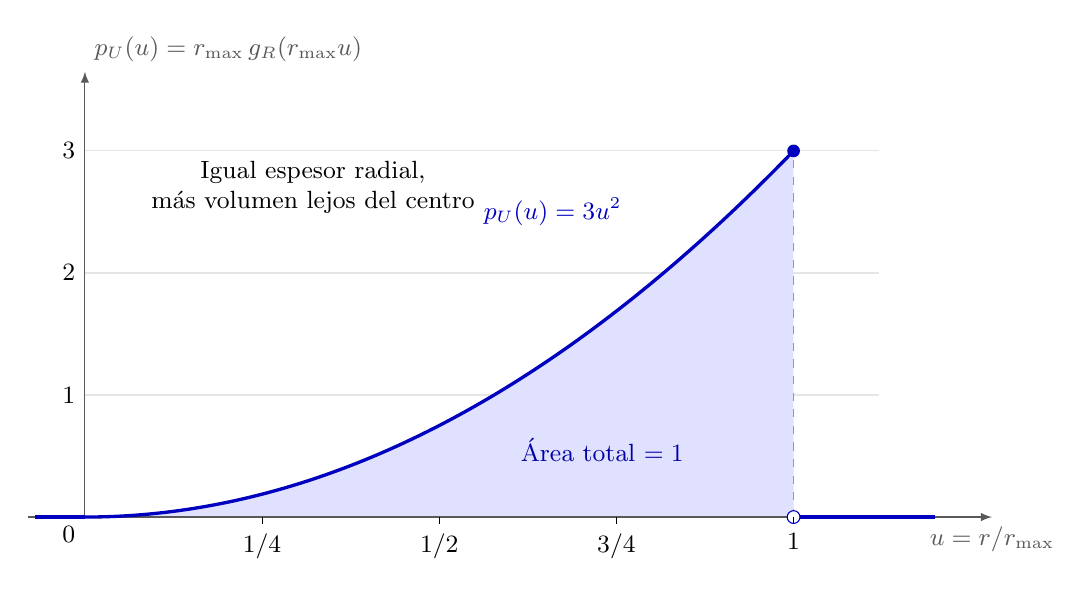
\begin{tikzpicture}[x=9cm,y=1.55cm,font=\small,>=latex]
  \foreach \level in {1,2,3}{
    \draw[black!10] (0,\level) -- (1.12,\level);
    \node[left] at (0,\level) {$\level$};
  }
  \fill[blue!12] (0,0) -- plot[domain=0:1,samples=90,variable=\radiusvalue]
    ({\radiusvalue},{3*\radiusvalue*\radiusvalue}) -- (1,0) -- cycle;
  \draw[->,black!65] (-0.08,0) -- (1.28,0) node[below] {$u=r/r_{\max}$};
  \draw[->,black!65] (0,0) -- (0,3.65) node[above right] {$p_U(u)=r_{\max}\,g_R(r_{\max}u)$};
  \draw[blue!75!black,very thick] plot[domain=0:1,samples=90,variable=\radiusvalue]
    ({\radiusvalue},{3*\radiusvalue*\radiusvalue});
  \draw[blue!75!black,very thick] (-0.07,0) -- (0,0);
  \draw[blue!75!black,very thick] (1,0) -- (1.2,0);
  \draw[dashed,black!40] (1,0) -- (1,3);
  \fill[blue!75!black] (1,3) circle (2.3pt);
  \draw[blue!75!black,fill=white] (1,0) circle (2.3pt);
  \foreach \tick/\labelvalue in {0.25/{1/4},0.5/{1/2},0.75/{3/4},1/1}{
    \draw (\tick,0) -- (\tick,-0.055) node[below] {$\labelvalue$};
  }
  \node[below left] at (0,0) {$0$};
  \node[text=blue!75!black] at (0.66,2.5) {$p_U(u)=3u^2$};
  \node[align=center,text=blue!65!black] at (0.73,0.55) {Área total $=1$};
  \node[align=center,anchor=west] at (0.08,2.7) {Igual espesor radial,\\más volumen lejos del centro};
\end{tikzpicture}
\shorthandon{<>}
\caption{Densidad de la distancia en la escala $U=R/r_{\max}$. La curva crece cuadráticamente dentro de la esfera y la densidad es cero fuera de ella. El área sombreada representa toda la probabilidad. La línea vertical discontinua sólo señala el borde $r=r_{\max}$; no forma parte de la densidad.}
\label{fig:densidad-distancia-estelar}
\end{figure}